\documentclass{article}

\usepackage{fancyhdr}
\usepackage{extramarks}
\usepackage{amsmath}
\usepackage{amsthm}
\usepackage{amsfonts}
\usepackage{tikz}
\usepackage[plain]{algorithm}
\usepackage{algpseudocode}
\usepackage{xcolor}
\usepackage{enumitem}
\usepackage{amssymb}
\usepackage{todonotes}
\usepackage{mathtools}

\usetikzlibrary{automata,positioning}

%
% Basic Document Settings
%

\topmargin=-0.45in
\evensidemargin=0in
\oddsidemargin=0in
\textwidth=6.5in
\textheight=9.0in
\headsep=0.25in

\linespread{1.1}

\pagestyle{fancy}
\lhead{\hmwkAuthorName}
\chead{\hmwkClass\ (\hmwkClassInstructor): \hmwkTitle}
\rhead{\firstxmark}
\lfoot{\lastxmark}
\cfoot{\thepage}

\renewcommand\headrulewidth{0.4pt}
\renewcommand\footrulewidth{0.4pt}

\setlength\parindent{0pt}

%
% Create Problem Sections
%

\newcommand{\enterProblemHeader}[1]{
    \nobreak\extramarks{}{Problem \arabic{#1} continued on next page\ldots}\nobreak{}
    \nobreak\extramarks{Problem \arabic{#1} (continued)}{Problem \arabic{#1} continued on next page\ldots}\nobreak{}
}

\newcommand{\exitProblemHeader}[1]{
    \nobreak\extramarks{Problem \arabic{#1} (continued)}{Problem \arabic{#1} continued on next page\ldots}\nobreak{}
    \stepcounter{#1}
    \nobreak\extramarks{Problem \arabic{#1}}{}\nobreak{}
}

\newcount\colveccount
\newcommand*\colvec[1]{
        \global\colveccount#1
        \begin{pmatrix}
        \colvecnext
}
\def\colvecnext#1{
        #1
        \global\advance\colveccount-1
        \ifnum\colveccount>0
                \\
                \expandafter\colvecnext
        \else
                \end{pmatrix}
        \fi
}

\setcounter{secnumdepth}{0}
\newcounter{partCounter}
\newcounter{homeworkProblemCounter}
\setcounter{homeworkProblemCounter}{1}
\nobreak\extramarks{Problem \arabic{homeworkProblemCounter}}{}\nobreak{}

%
% Homework Problem Environment
%
% This environment takes an optional argument. When given, it will adjust the
% problem counter. This is useful for when the problems given for your
% assignment aren't sequential. See the last 3 problems of this template for an
% example.
%
\newenvironment{homeworkProblem}[1][-1]{
    \ifnum#1>0
        \setcounter{homeworkProblemCounter}{#1}
    \fi
    \section{Problem \arabic{homeworkProblemCounter}}
    \setcounter{partCounter}{1}
    \enterProblemHeader{homeworkProblemCounter}
}{
    \exitProblemHeader{homeworkProblemCounter}
}

%
% Homework Details
%   - Title
%   - Due date
%   - Class
%   - Section/Time
%   - Instructor
%   - Author
%

\newcommand{\hmwkTitle}{Homework 1}
\newcommand{\hmwkDueDate}{February 27, 2018}
\newcommand{\hmwkClass}{Discrete Structures}
\newcommand{\hmwkClassTime}{Spring Semester}
\newcommand{\hmwkClassInstructor}{Prof. Stefan Wolf}
\newcommand{\hmwkAuthorName}{\textbf{Romanelli / Lunardi}}

%
% Title Page
%

\title{
    \vspace{2in}
    \textmd{\textbf{\hmwkClass:\ \hmwkTitle}}\\
    \normalsize\vspace{0.1in}\small{Due\ on\ \hmwkDueDate\ at 10:30am}\\
    \vspace{0.1in}\large{\textit{\hmwkClassInstructor}}
    \vspace{3in}
}

\author{\hmwkAuthorName}
\date{}

\renewcommand{\part}[1]{\textbf{\large Part \Alph{partCounter}}\stepcounter{partCounter}\\}

%
% Various Helper Commands
%

% Useful for algorithms
\newcommand{\alg}[1]{\textsc{\bfseries \footnotesize #1}}

% For derivatives
\newcommand{\deriv}[1]{\frac{\mathrm{d}}{\mathrm{d}x} (#1)}

% For partial derivatives
\newcommand{\pderiv}[2]{\frac{\partial}{\partial #1} (#2)}

% Integral dx
\newcommand{\dx}{\mathrm{d}x}

% Alias for the Solution section header
\newcommand{\solution}{\textbf{\large Solution}}

% Probability commands: Expectation, Variance, Covariance, Bias
\newcommand{\E}{\mathrm{E}}
\newcommand{\Var}{\mathrm{Var}}
\newcommand{\Cov}{\mathrm{Cov}}
\newcommand{\Bias}{\mathrm{Bias}}

\begin{document}

\maketitle

\pagebreak

\begin{homeworkProblem}
  For this problem let's consider the following checkboard:
  \begin{figure}[h]
    \centering
    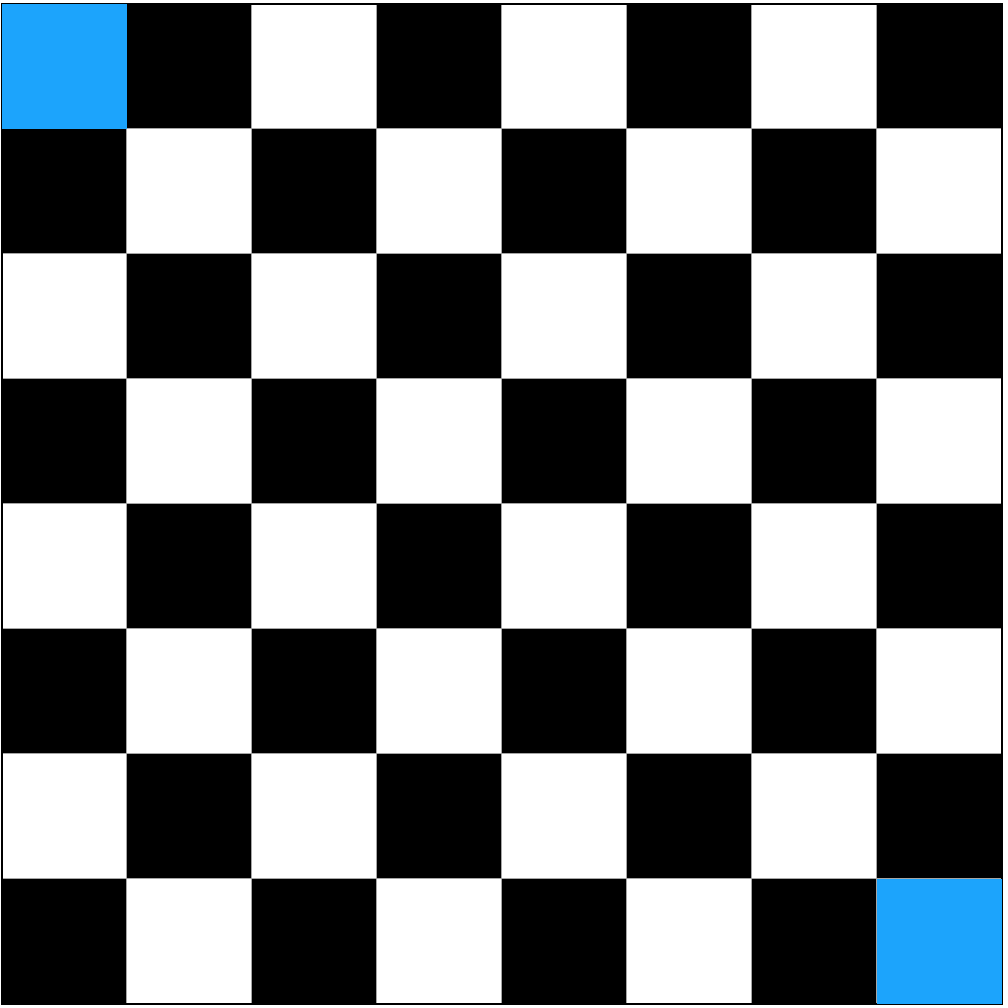
\includegraphics[width=5cm]{media/checkboard.png}
  \end{figure} \\
  Where the top-left and the bottom-right cells have been removed. \\ \\
  Now we must consider that whenever we place down a domino piece, we will undoubtedly cover two cells and because of how a chessboard is organised, that is, since there are never two adjacent cells that have the same color, this must mean that the domino piece will necessarily go over a black and a white cell, just like here below:
  \begin{figure}[h]
    \centering
    
\includegraphics[width=5cm]{media/domino.png}
  \end{figure} \\
  Having 32 white cells and 32 black cells in a 8x8 chessboard, this allows us indeed to place down 32 domino pieces but, since the two cells that we just removed are white, a problem occurs: the chessboard is now composed by 32 black cells and 30 white cells, and one would be justified to think that they could still be filled with 31 domino pieces, however, if we reckon what we just said above, a domino piece will have to occupy a white cell as well as a black one. \\ \\
  This will leave us at the end with 2 black cells left to fill, which constitutes a problem for us: the two cells will, by definition, never be adjacent and thus a domino piece will never be able to fit in the two gaps left.
  \begin{figure}[h]
    \centering
    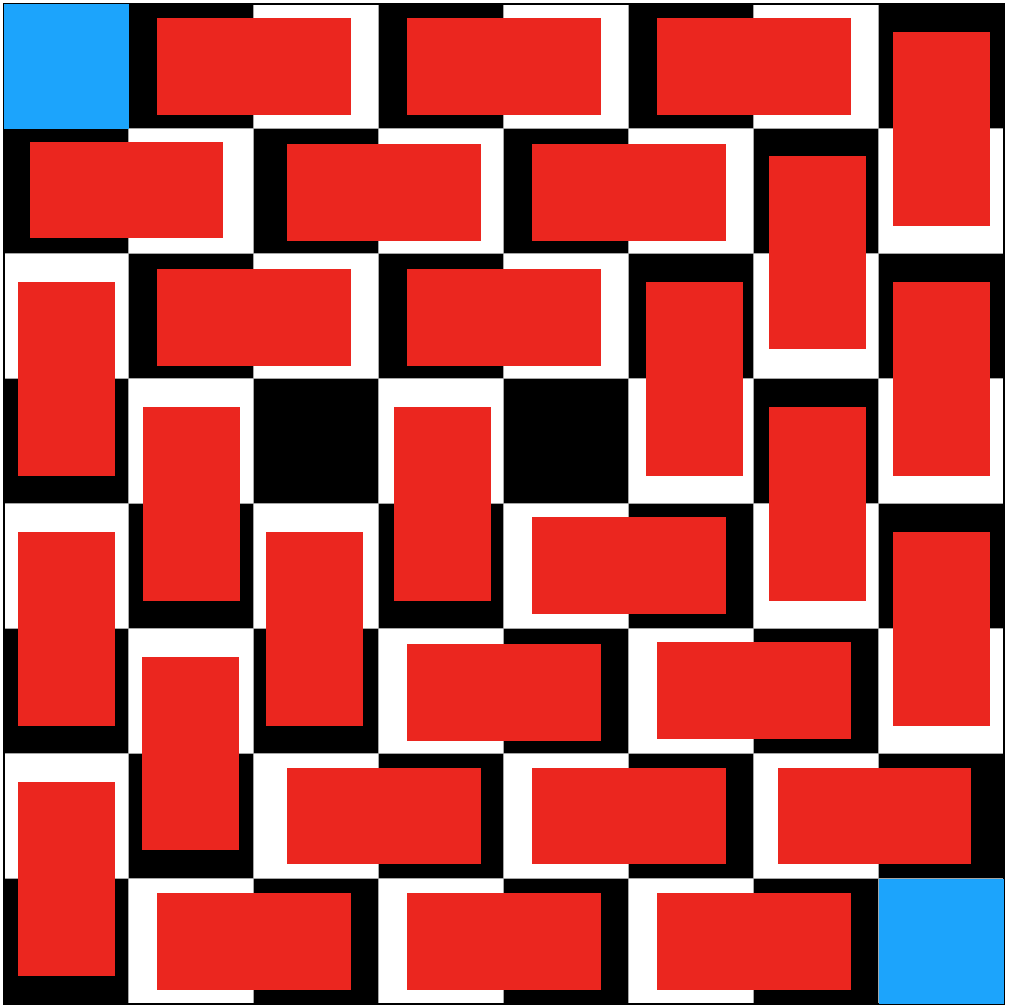
\includegraphics[width=5cm]{media/impossibru.png}
  \end{figure}
\end{homeworkProblem}
\newpage
\begin{homeworkProblem}
  For this problem, we are asked to split a \emph{Rubik's Cube} into its 27 smaller cube that compose it. \\
  Now we are asked if it is possible, by means of cutting and reorganising the cube, to isolate all of the smaller cubes with less than six cuts, but that's impossible! \\ \\
  \begin{figure}[h]
    \centering
    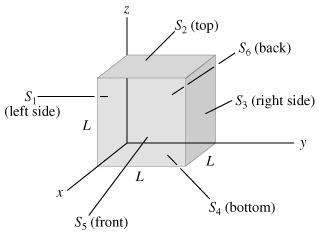
\includegraphics[width=8cm]{media/cube.jpg}
  \end{figure}
  The reason behind this is fairly simple: in order to cut out the innermost cube, which we can consider to be the 27th, the other 26 cubes being the ones visible from the outside, it is not possible to isolate that one without cutting along all of its faces, which for a cube, as we all know, are six.

\end{homeworkProblem}
\newpage
\begin{homeworkProblem}
  We are given the following group of six people, $S:= {A, B, C, D, E, F}$, we want to show that in any possible case, it's always true that at least one of the two following statements is verified: \\
  \vspace{-0.5cm}
  \begin{itemize}
    \item[\textbf{a)}] There are three people which have never shaken hands with each other.\\
    \vspace{-0.5cm}
    \item[\textbf{b)}] There are three people which all already have shaken hands with each other.
  \end{itemize}
  The question is simply whether we can always find at least one triangle composed by elements connected with each other, or not connected. \\ \\
  Let's rearrange the nodes in a simple way and connect all of them with each other without creating any monochromatic triangle. \\
  We start off by connecting all the nodes to a common element, that being A:
  \begin{figure}[h]
    \centering
    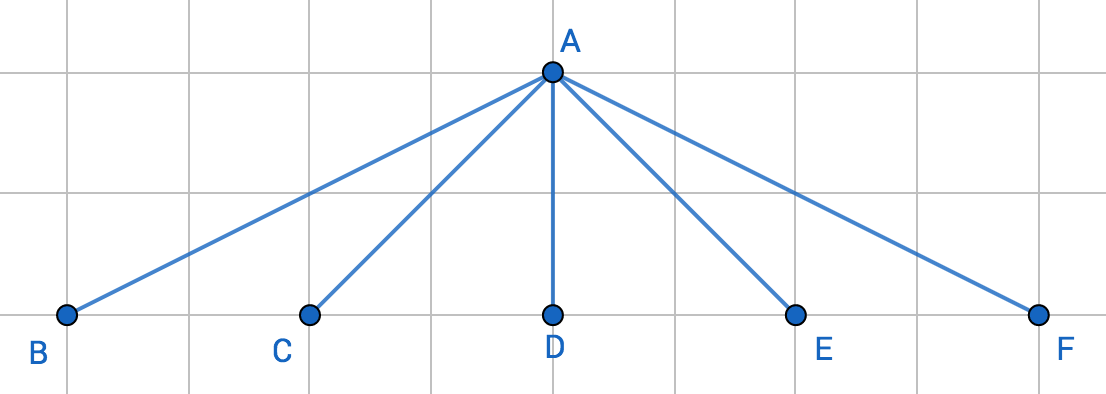
\includegraphics[width=0.6\textwidth]{media/part1.png}
  \end{figure} \\
  Now, in order not to create a monochromatic triangle, for instance $\widehat{ABC}$, we need to connect $\overline{BC}$ with a red line and the same goes for $\widehat{ACD}$ with $\overline{CD}$.
  \begin{figure}[h]
    \centering
    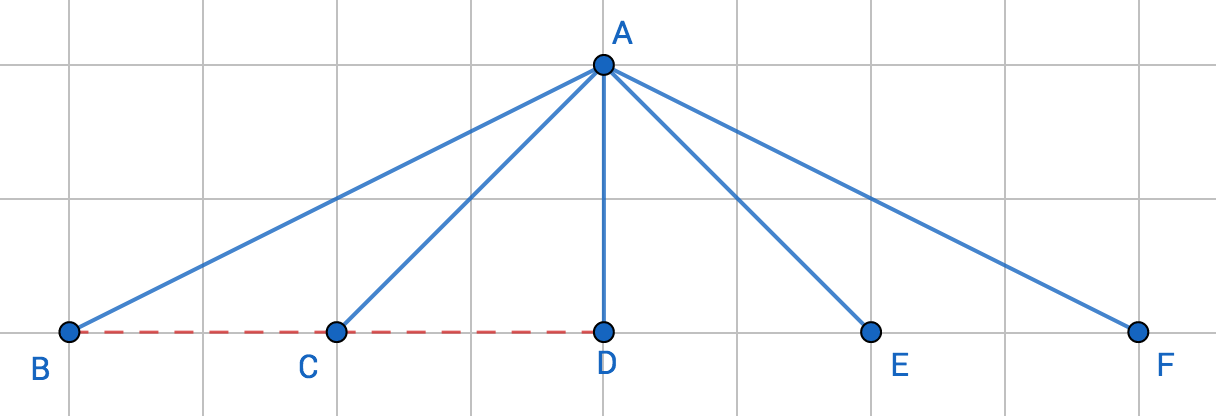
\includegraphics[width=0.6\textwidth]{media/part2.png}
  \end{figure} \\
  Finally, we should now avoid connecting the triangle $\widehat{ABD}$, by connecting $\overline{BD}$ with a red line. But this is not so trivial, since doing so will create the "triangle" $\widehat{BCD}$ of the opposite color.
  \begin{figure}[h]
    \centering
    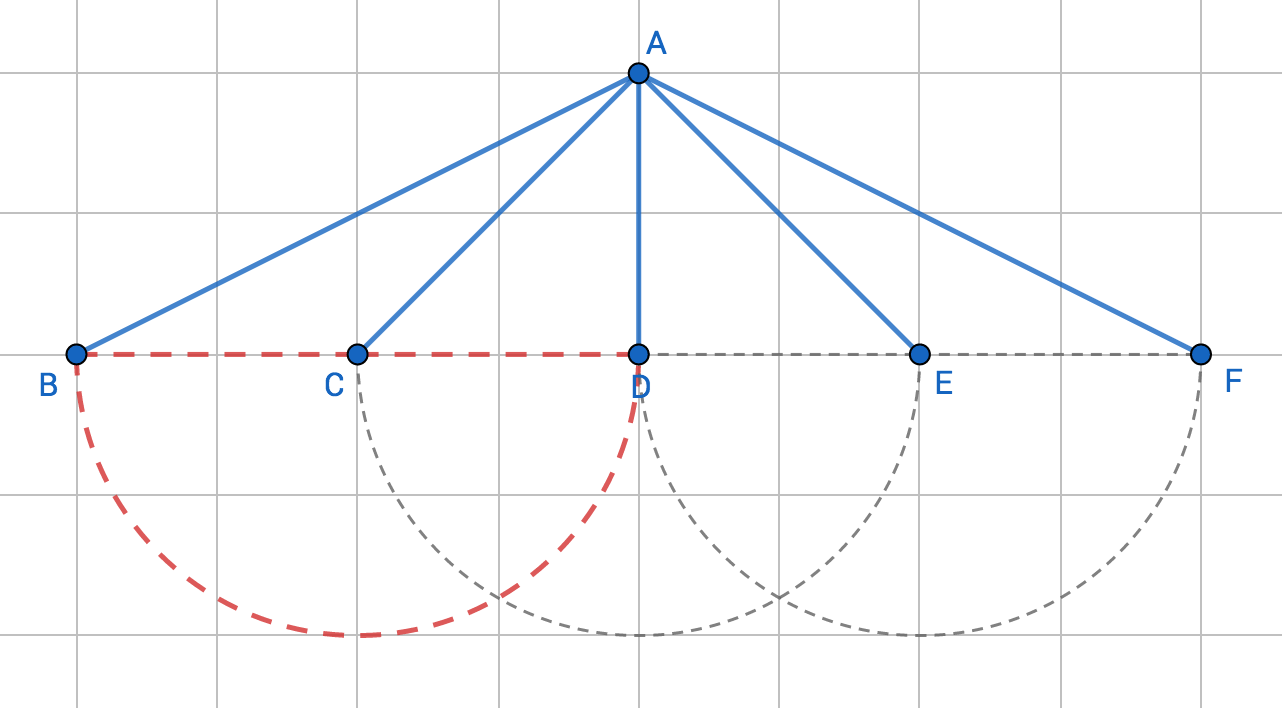
\includegraphics[width=0.6\textwidth]{media/part3.png}
  \end{figure} \\
  This is really bad news, because it means that there is no possible way of getting away with this: no matter what we do, we will always end up with closing a monochromatic triangle, even if we change the initial configuration!
\end{homeworkProblem}

\begin{homeworkProblem}
  We are going to consider n points in the plane, so that whenever we connect two points, at least one additional point must lie on the line. We want to show that if this is the case, all points line on the same line. \\ \\
  The following is a representation of such statement:
  \begin{figure}[h]
    \centering
    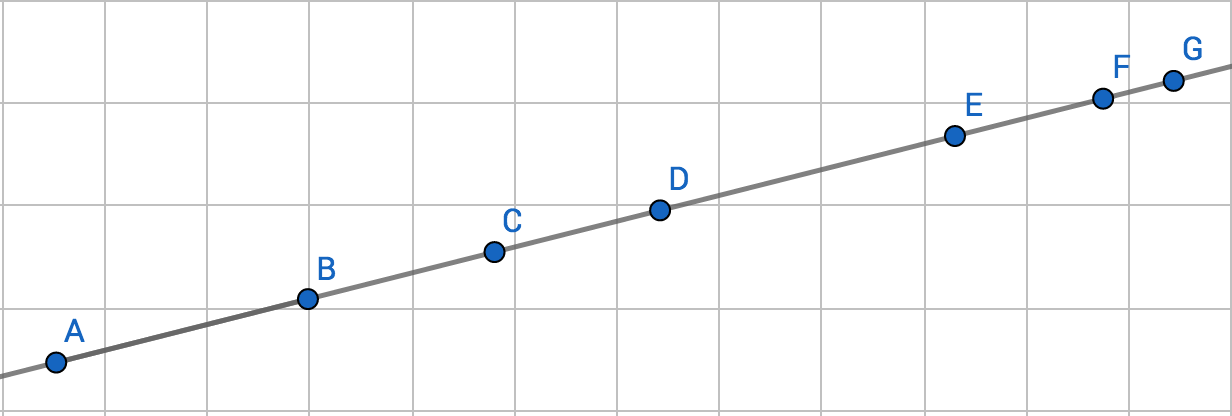
\includegraphics[width=0.5\textwidth]{media/line.png}
  \end{figure} \\
  Now, the problem points us toward finding a contradiction by assuming that the statement is false, hence we get something that looks like this:
  \begin{figure}[h]
    \centering
    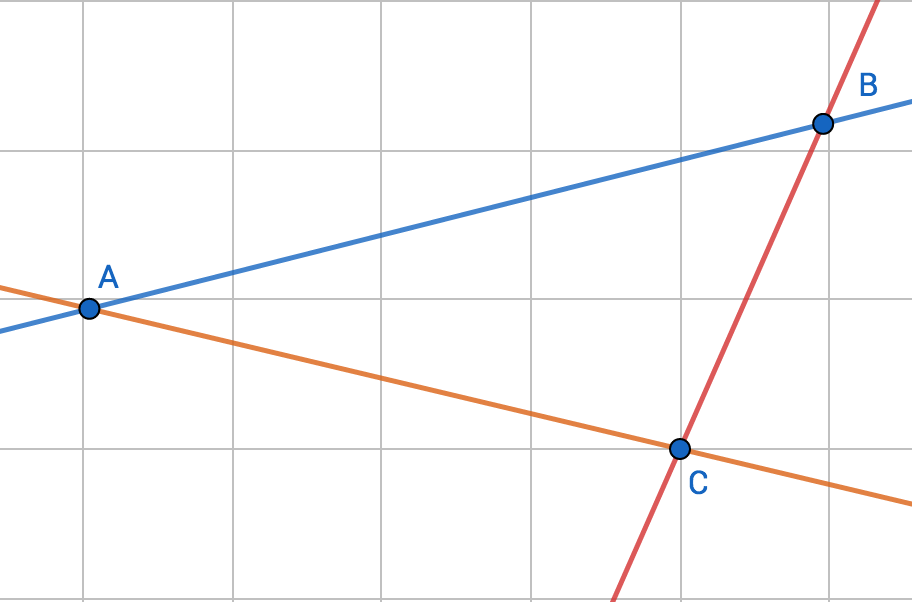
\includegraphics[width=0.4\textwidth]{media/lines.png}
  \end{figure} \\
  At this point it does not really matter whether we want to connect and create a new line between $A$ and $C$ or $B$ and $C$. By connecting two points we are inevitably creating a third point, that if we now connect to an existing one, will create a new line, triggering over and over the same behavior.
  \begin{figure}[h]
    \centering
    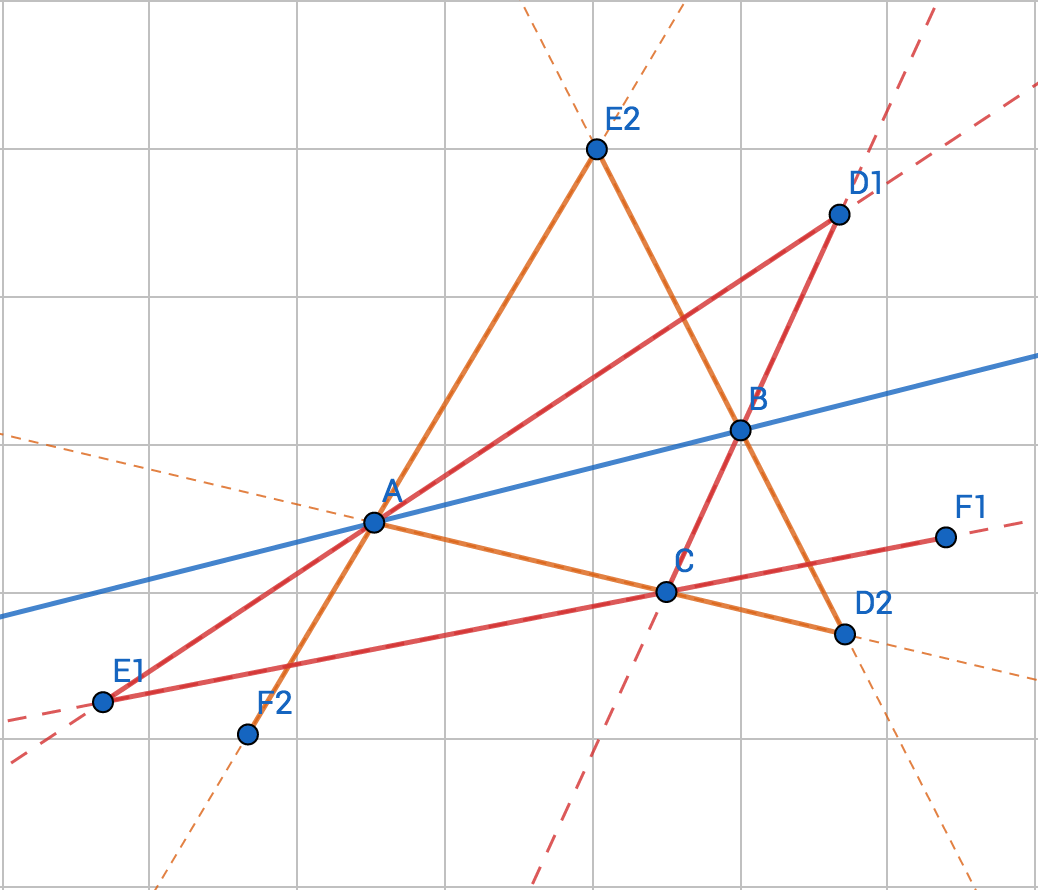
\includegraphics[width=0.35\textwidth]{media/path.png}
  \end{figure} \\
  Since for any new point in the sequence $A, C, D2, E2, F2, ..., n$ or $B, C, D1, E1, F1, ..., n$ a new line is created, we can deduce that the points won't lie on the same line. Hence it's necessary that the third point lies on the same line as the other previous two, at any given connection to avoid this scenario.
\end{homeworkProblem}

\end{document}
